%-/***************************************************************************/
%-/* This file is part of FERRET, an add-on module for MOOSE
%-
%-/* FERRET is free software: you can redistribute it and/or modify
%-   it under the terms of the GNU General Public License as published by
%-   the Free Software Foundation, either version 3 of the License, or
%-  (at your option) any later version.

%-/* This program is distributed in the hope that it will be useful,
%-   but WITHOUT ANY WARRANTY; without even the implied warranty of
%-   MERCHANTABILITY or FITNESS FOR A PARTICULAR PURPOSE. See the
%-   GNU General Public License for more details.
%-
%-/* You should have received a copy of the GNU General Public License
%-   along with this program.  If not, see <http://www.gnu.org/licenses/>.
%-
%-   For help with FERRET please contact J. Mangeri <john.mangeri@uconn.edu>
%-   and be sure to track new changes at bitbucket.org/mesoscience/ferret
%-
%-/****************************************************************************/
%----------------------------------------------------------------------------------------
%	PACKAGES AND OTHER DOCUMENT CONFIGURATIONS
%----------------------------------------------------------------------------------------

\documentclass[22pt]{article} % Default font size is 12pt, it can be changed here

\usepackage[margin=0.75in, centering]{geometry} % Required to change the page size to A4
% Set the page size to be A4 as opposed to the default US Letter

\usepackage{graphicx} % Required for including pictures
\usepackage{amsmath}
\usepackage{float} % Allows putting an [H] in \begin{figure} to specify the exact location of the figure
\usepackage{wrapfig} % Allows in-line images such as the example fish picture
\usepackage{subfigure}
\usepackage{hyperref}
\usepackage[mathscr]{euscript}
\usepackage{lipsum} % Used for inserting dummy 'Lorem ipsum' text into the template
\usepackage[english]{babel}

\usepackage{dsfont} %for fancy identity matrices \mathds{1}
\usepackage[utf8]{inputenc}
\usepackage{fancyhdr}
 
\pagestyle{fancy}
\fancyhf{}
\rhead{\textsc{Ferret} \textbf{unofficial} notes}
\lhead{}
\rfoot{Page \thepage}


\linespread{1.5} % Line spacing

%\setlength\parindent{0pt} % Uncomment to remove all indentation from paragraphs

\begin{document}

%%----------------------------------------------------------------------------------------
%%	TITLE PAGE
%%----------------------------------------------------------------------------------------
%
%\begin{titlepage}
%
%
%\end{titlepage}

%----------------------------------------------------------------------------------------
%	TABLE OF CONTENTS
%----------------------------------------------------------------------------------------

\tableofcontents % Include a table of contents

\newpage % Begins the essay on a new page instead of on the same page as the table of contents 

%----------------------------------------------------------------------------------------
%	INTRODUCTION
%----------------------------------------------------------------------------------------
\large

\section{Introduction}

\subsection{Elastic problem}

%
\paragraph{}We first consider a polarizable linear elastic body, $\Omega$, under some crystallographic misfit strain, $\varepsilon_{ij}^\mathrm{misfit} (\textbf{r})$.
%
Einstein summation notation is assumed throughout this document.
%
Above the Curie temperature, $T_C$, the polarization, $\textbf{P}$, is zero. 
%
Thus, the total elastic free energy of the system is, 
%
\begin{equation}\tag{1}
F_\mathrm{elastic} = \int\limits_\Omega d^3 \textbf{r} \,\,\, f_\mathrm{elastic} = \int\limits_\Omega d^3 \textbf{r} \,\,\, C_{ijkl} \left(\varepsilon_{ij} - \varepsilon_{ij}^\mathrm{misfit} \right) \left(\varepsilon_{kl} - \varepsilon_{kl}^\mathrm{misfit} \right) 
\end{equation}
%
where 
%
\begin{equation}\tag{2}
\varepsilon_{ij} = \frac{1}{2} \left(\frac{\partial u_i}{\partial x_j} + \frac{\partial u_j}{\partial x_i} \right)
\end{equation}
%
and with the elastic stiffness tensor $C_{ijkl}$ being of rank four that obeys material symmetry \cite{NyeBook}.
%

%
Note that $u_i =  u_i (\textbf{r})$, are the displacement vectors.
%
Under mechanical equilibrium, the system obeys,
%
\begin{wrapfigure}{r}{0.5\textwidth}
  \begin{center}
\vspace{-12pt}
    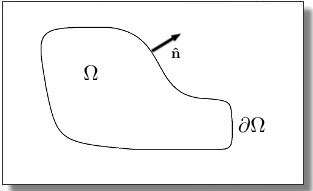
\includegraphics[width=0.475\textwidth]{geometry.jpg}
  \end{center}
  \caption{Geometry setup in \textsc{Ferret}.
%
$\Omega$ is completely bounded by surface $\partial \Omega$. $\hat{\textbf{n}}$ is an \emph{outward} facing surface normal.
%
The volume and the surface may exist as set of subdomains, $\Omega_k \subseteq \Omega_{k+1} \subseteq ... \subseteq \Omega$ and $\partial \Omega_k \subseteq \partial \Omega_{k+1} \subseteq ... \subseteq \partial \Omega$.
%
This block decomposition proves useful when defining the material properties of the problem.} %it should be noted that Moose will rename this to "subdomain" instead of block in the near future
\end{wrapfigure}
%
%
\begin{equation}\tag{3}
0 = \frac{\partial F}{\partial u_i} \Rightarrow \sigma_{ij,j} = \frac{\partial}{\partial x_j} C_{ijkl} \left(\varepsilon_{kl} - \varepsilon_{kl}^\mathrm{misfit} \right) = 0,
\end{equation}
%
the so-called stress-divergence equation \cite{Morton1975, BowerBook}.
%

%
\subsubsection{Surface elastic problem}
%
\paragraph{}In a elastic material, a surface tension can arise from a free surface, $\partial \Omega$, bounding the body, $\Omega$.
%
Here, this surface tension, with the Gurtin-Murdoch approach \cite{Morton1975},  is related to surface tensorial quantities by
%
\begin{equation}\tag{3.1}
\sigma_{\alpha \beta}^s = \tau^0 \delta_{\alpha \beta} + C_{\alpha \beta \delta \gamma}^s \varepsilon_{\delta \gamma}^s
\end{equation}
%
where $\alpha, \beta, \gamma, \delta = 1,2$ denote crystallographic directions along the surface.
%
$C_{\alpha \beta \delta \gamma}^s$ is the surface elastic tensor, and $\varepsilon_{\delta \gamma}^s$ is a surface elastic strain. The surface elastic tensor obeys the minor symmetries $C_{\alpha \beta \gamma \delta}^s = C_{\alpha \beta \delta \gamma }^s$ and $C_{\alpha \beta \delta \gamma}^s = C_{\beta \alpha \delta \gamma }^s$ and therefore has at most nine independent components.
%
The tension, $\tau^0$ is the intrinsic surface tension.
%
A surface free energy, $F_\mathrm{surface}$ can be introduced as,
%
\begin{equation}\tag{3.5}
F_\mathrm{surface} = \frac{1}{2} \int\limits_{\delta \Omega} d^2 \textbf{r} \,\,\, C_{\alpha \beta \delta \gamma }^s \varepsilon_{\alpha \beta}^s \varepsilon_{\delta \gamma}^s 
\end{equation}
%
with
%
\begin{equation}\tag{3.6}
 \varepsilon_{\alpha \beta}^s = \frac{1}{2} \left(\frac{\partial u_\alpha}{\partial x_\beta} + \frac{\partial u_\beta}{\partial x_\alpha} \right).
\end{equation}
%
The purely elastic free energy balance of the volume $\Omega$ bounded by $\delta \Omega$ with body forces $\textbf{b}$ and traction $\tau$ upon the surface, under an infinitesimal displacement field $\textbf{u}$, is
%
\begin{align}\tag{3.7}
 \frac{1}{2} \int\limits_\Omega C_{ijkl} \varepsilon_{ij} \varepsilon_{kl} \,\,d^3 \textbf{r} + \frac{1}{2} \int\limits_{\delta \Omega} \,\, C_{\alpha \beta \delta \gamma}^s \varepsilon_{\alpha \beta}^s \varepsilon_{\delta \gamma}^s\,\, d^2 \textbf{r} = \int\limits_\Omega \textbf{b} \cdot \textbf{u} \,\,\,d^3 \textbf{r} + \int\limits_{\partial \Omega} \tau \cdot \mathbf{\hat{n}} \,\,d^2 \textbf{r} - \int\limits_{\partial \Omega} \tau^0_{\alpha \beta} \varepsilon_{\alpha \beta}^s \,\,d^2 \textbf{r} \\ \nonumber
\end{align}
%
for some surface normal $\mathbf{\hat{n}}$.
%
Enforcing stationary under first-order variations \cite{BowerBook}, gives us three $(k = 1,2,3)$ weak form of the equations suitable for Galerkin finite element analysis, with test function $\psi_h$:
%
\begin{align}\tag{3.8}
 0 = \int\limits_\Omega C_{ijkl} \frac{\partial u_i}{\partial x_j} \frac{\partial \psi_h}{\partial x_l} d^3 \textbf{r} + \int\limits_{\partial \Omega} C_{ijkl}^s \left(\frac{\partial u_i}{\partial x_j} \frac{\partial \psi_h}{\partial x_k} \right)_s d^2 \textbf{r} - \int\limits_\Omega b_k \psi_h d^3 \textbf{r} - \int\limits_{\partial \Omega} \tau_k \psi_h d^2 \textbf{r} + \int\limits_{\partial \Omega} \left(\tau_{ij}^0 \frac{\partial \psi_h}{\partial x_j} \right)_s d^2 \textbf{r}.
\end{align}
%
The notation $\left( . \right)_s$ denotes the projection of the tensor onto the surface.
%
These quantities are constructed and each quadrature point on the finite element mesh surface by taking their bulk counterparts and using a local projection operator $\mathbf{\hat{\textbf{D}}} = \mathds{1} - \mathbf{\hat{n}}(\textbf{r}) \otimes \mathbf{\hat{n}} (\textbf{r})$ \cite{Yvonnet2012} such that 
%
\begin{align}\tag{3.9}
\sigma^s = \mathbf{\hat{\textbf{D}}} \sigma \mathbf{\hat{\textbf{D}}} \,\,\,\mathrm{and}\,\,\, \varepsilon^s = \mathbf{\hat{\textbf{D}}} \varepsilon \mathbf{\hat{\textbf{D}}}.
\end{align}
%
For application of this technique, see Influence of Elastic and Surface Strains on the Optical Properties of Semiconducting Core-Shell Nanoparticles,
John Mangeri, Olle Heinonen, Dmitry Karpeyev, and Serge Nakhmanson, Phys. Rev. Applied 4, 014001 -- \href{http://journals.aps.org/prapplied/abstract/10.1103/PhysRevApplied.4.014001}{Published}  7 July 2015. 
%

%
\subsection{Ferroelectric materials below $T_C$}
%

%
\paragraph{}A distinct feature of ferroelectric materials is their ability to form polar domains under certain conditions.
%
As the material is cooled down below the Curie temperature, its local polarization evolves towards thermodynamic equilibrium.
%
In the absence of an applied field (or some other ordering influence), the stationary state of the polarization distribution throughout the material is usually a complex equilibrium pattern\footnote[1]{Which is not the true global energy minimum of the system, but rather a local metastable energy minimum \cite{Hu1998}.} pattern, known as the \emph{domain structure}.
%
An important technical question, that was originally highlighted by Hu and Chen \cite{Hu1998, Li2001}, is how one can predict the equilibrium inhomogeneous ferroelectric microstructure --- or the `shape' of the polarization field $\mathbf{P}(\mathbf{r})$ --- while making no particular assumptions about its initial state?
%
Following the work of Su and Landis \cite{Su2007} and starting from the elementary second law of thermodynamics\footnote[2]{The second law states that the total entropy of an isolated system can only increase in time.
%
Mathematically, it can be written as
%
$$dS > dQ/T$$
%
for entropy $S$, temperature $T$, and heat $Q$.
%
Implicit within this statement is that the process is irreversible, which is the case of the domain structure formation as ferroic material is cooled below $T_C$.}, one can derive a time-dependent equation describing the evolution of $\mathbf{P}(\mathbf{r})$ that has the form of the celebrated Allen-Cahn equation \cite{Chan1977, LandauBook, Allen1979}.
%
%
\begin{align}\label{eq:time-dependent_landau_ginzburg_devonshire}
\frac{\partial P_i}{\partial t} = -\Gamma \frac{\delta }{\delta P_i}\Bigg(F\left[P_i\right] \Bigg)\,\,\mathrm{for} \,\,i = 1,2,3,
\end{align}
%
where the term in brackets is the variational derivative \footnote[3]{Variational derivative (sometimes called functional derivative) relates a change in a functional to a change in the function that functional depends on.
%
Let
%
$$J[f] = \int L[x,f,f'] dx,$$
%
where $J$ is a functional of $L$ that depends on $f = f(x)$, with $f'$ being the derivative of $f$ with respect to $x$. Then
%
$$\frac{\delta J}{\delta f} = \frac{\partial L}{\partial f} - \frac{d}{dx} \frac{\partial L}{\partial f'}.$$
%
This is also known as the Euler-Lagrange equation, if equated to zero \cite{GelfandBook}.
} with respect to $P_i$.
%
This equation is known as the time-dependent Landau-Ginzburg-Devonshire equation (TDLGD) and can be used to predict, with some general assumptions about initial conditions, the equilibrium polar domain structure within a ferroelectric system at a given temperature and elastic/electric boundary conditions.
%

%
The value of $\Gamma$ that has to be adopted for generic ferroelectric materials is still a subject of an extensive debate. Some researchers have suggested that $\Gamma$ can depend on the strength of the applied electric field during hysteretic switching \cite{Meng2015}.
%
Reasonable assumptions about $\Gamma$ for certain poling scenarios have produced good agreement with experimental results, such as the coercive field magnitudes and relaxation times of the polar field \cite{Fridkin2000, Hlinka2007}.
%
The total energy, $F$, can be written as an integral over a linear combination of energy densities,
%
$$F = \int\limits_\Omega d^3 \textbf{r} \Bigg[f_\mathrm{bulk} + f_\mathrm{elastic} + f_\mathrm{elec} + f_\mathrm{grad} \Bigg].$$
%
In standard fashion, the bulk free energy density, $f_\mathrm{bulk}$ is expanded to sixth order,
%
$$f_\mathrm{bulk} = \alpha_{i} P_i + \beta_{ij} P_i P_j + \gamma_{ijk} P_i P_j P_k + \delta_{ijkl} P_i P_j P_k P_l  + \epsilon_{ijklm} P_i P_j P_k P_l P_m + \zeta_{ijklmn} P_i P_j P_k P_l P_m P_n.$$
%
The elastic energy density, 
%
$$f_\mathrm{elastic} = \frac{1}{2} C_{ijkl} \left(\varepsilon_{ij} - \varepsilon_{ij}^0 \right) \left(\varepsilon_{kl} - \varepsilon_{kl}^0 \right) $$
%
contains the stress-free strain
%
$$\varepsilon_{kl}^0 = Q_{klmn} P_m P_n,$$
%
that arises due to the polarization for some electrostrictive coefficient tensor, $Q_{ijkl}$, of rank four. 
%
Note that this term can be decomposed into two terms (one of which explicitly contains the polarization field).
%
The electrostatic energy density term is written in the following fashion, 
%
\begin{align}\nonumber
f_\mathrm{electrostatic} &= - \frac{1}{2} E_k D_k\\ \nonumber
&= \frac{1}{2} \frac{\partial \Phi_\mathrm{int}}{\partial x_k} D_k\\ \nonumber
&= \frac{1}{2} \frac{\partial \Phi_\mathrm{int}}{\partial x_k} \left[- \epsilon_b \epsilon_0 \frac{\partial \Phi_\mathrm{int}}{\partial x_k}  + P_k\right]\\ \nonumber
\end{align}
%
using $E_k = - \partial \Phi_\mathrm{int} / \partial x_k$ and $D_k = \epsilon_b \epsilon_0 E_k + P_k$ with $\Phi_\mathrm{int}$ being the internal\footnote[4]{The factor of $\frac{1}{2}$ being physically significant due to the adiabatic charging of the capacitor} electrostatic potential generated by the Poisson equation,
%
$$\frac{\partial}{\partial x_j} \left( \epsilon_b \epsilon_0 \frac{\partial \Phi_\mathrm{int}}{\partial x_j}\right) = - \frac{\partial P_k}{\partial x_k}.$$
%
The parameter $\epsilon_b$ is the dielectric constant of the ferroelectric medium due to the core-electrons (sometimes noted as $\epsilon^\infty$ in DFT routines).
%
For the purposes of perovskite-ferroelectrics, $\epsilon_b$ is about $5-10$ in units of vacuum permittivity. 
%
Externally to the ferroelectric medium, 
%
$$\frac{\partial}{\partial x_j} \left( \epsilon_{b,e} \epsilon_0 \frac{\partial \Phi_\mathrm{int}}{\partial x_j}\right) = 0$$
%
where the subscript $b,e$ denotes the (optical) dielectric constant of the external medium in units of $\epsilon_0$.
%
The energy density due to local gradients of the polarization, usually called the Ginzburg functional is, 
%
$$f_\mathrm{grad} = G_{ijkl} \frac{\partial P_i}{\partial x_j} \frac{\partial P_k}{\partial x_l}.$$
%

%
\subsection{The case of the proper cubic-tetragonal phase transition}
%

%
\paragraph{}The coefficient tensors, $\alpha_{i}$, $\beta_{ij}$, $\gamma_{ijk}$, $\delta_{ijkl}$, $\epsilon_{ijklm}$, $\zeta_{ijklmn}$, $G_{ijkl}$, and $Q_{mnkl}$,  and $C_{ijkl}$ are material dependent, obey symmetries of the lattice, and in general can be dependent at temperature, $T$.
%
Symmetrizing the energy density terms for the case of a cubic parent phase, one writes
%
\begin{align}\nonumber
f_\mathrm{bulk} &= \alpha_1 \left(P_x^2 + P_y^2 + P_z^2 \right) + \alpha_{11} \left(P_x^4 + P_y^4 + P_z^4 \right) + \alpha_{12} \left(P_x^2 P_y^2 + P_y^2 P_z^2 + P_x^2 P_z^2 \right) \\ \nonumber
&+ \alpha_{111} \left(P_x^6 + P_y^6 + P_z^6 \right) + \alpha_{112} \left[P_x^4 \left(P_y^2 + P_z^2 \right) + P_y^4 \left(P_x^2 + P_z^2 \right) + P_z^4 \left(P_x^2 + P_y^2 \right) \right] + \alpha_{123} \left(P_x^2 P_y^2 P_z^2 \right), \\ \nonumber
\end{align}
%
and
%
\begin{align}\nonumber
f_\mathrm{grad} &= \frac{1}{2} G_{11} \left[\left(\frac{\partial P_x}{\partial x} \right)^2 \hspace{-1pt}+\hspace{-1pt} \left(\frac{\partial P_y}{\partial y}\right)^2 \hspace{-1pt}+\hspace{-1pt}\left( \frac{\partial P_z}{\partial z} \right)^2\right] \\ \nonumber
&+ G_{12} \left[\frac{\partial P_x}{\partial x}\frac{\partial P_y}{\partial y}\hspace{-2pt} +\hspace{-1pt} \frac{\partial P_y}{\partial y} \frac{\partial P_z}{\partial z}\hspace{-2pt} +\hspace{-1pt} \frac{\partial P_x}{\partial x} \frac{\partial P_z}{\partial z} \right] \\ \nonumber
&+ \hspace{-2pt} \frac{1}{2} G_{44}  \hspace{-2pt}\left[\left(\frac{\partial P_x}{\partial y} \hspace{-1pt}+ \hspace{-1pt} \frac{\partial P_y}{\partial x} \right)^2 \hspace{-6pt}+\hspace{-2pt} \left(\frac{\partial P_y}{\partial z} \hspace{-1pt}+ \hspace{-1pt}\frac{\partial P_z}{\partial y} \right)^2 \hspace{-6pt}+\hspace{-2pt} \left(\frac{\partial P_x}{\partial z} \hspace{-1pt}+\hspace{-1pt} \frac{\partial P_z}{\partial x} \right)^2  \hspace{-0.5pt}\right] \\ \nonumber
&+ \hspace{-2pt}\frac{1}{2} G'_{44} \hspace{-2pt}\left[\left(\frac{\partial P_x}{\partial x_2} \hspace{-1pt}- \hspace{-1pt}\frac{\partial P_y}{\partial x} \right)^2 \hspace{-6pt} + \hspace{-2pt} \left(\frac{\partial P_y}{\partial z}\hspace{-1pt} - \hspace{-1pt}\frac{\partial P_z}{\partial y} \right)^2 \hspace{-6pt}+  \hspace{-2pt}\left(\frac{\partial P_x}{\partial z}\hspace{-1pt} - \hspace{-1pt}\frac{\partial P_z}{\partial x} \right)^2 \hspace{-0.5pt} \right].
\end{align}
%
with sign and factor of 2 convention from Ref. \cite{Li2001, Hlinka2006}.

%
%\section{Comments on the natural boundary condition of the paraelectric-ferroelectric interface}
%


%----------------------------------------------------------------------------------------
%	BIBLIOGRAPHY
%----------------------------------------------------------------------------------------
\begin{thebibliography}{1}
%\small{

\bibitem{Morton1975}
E.~Morton, G.~Gurtin, and A.~I.~Murdoch, 
%\newblock{A continuum theory of elastic material surfaces}
\newblock {\em Arch. Ration. Mech. Anal.} \textbf{57}, 291 (1975).

\bibitem{BowerBook}
A.~F.~Bower,
%\newblock {Applied Mechanics of Solids}.
\newblock \emph{Applied Mechanics of Solids.} CRC Press Inc. (2009).

\bibitem{NyeBook}
J.~F.~Nye,
%\newblock {Physical Properties of Crystals}.
\newblock \emph{Physical Properties of Crystals.} Oxford University Press Inc. (1985).

\bibitem{Yvonnet2012}
J.~Yvonnet, A.~Mitrushchenkov, G.~Chambaud, Q.-C.~He, and S.-T.~Gu, 
%\newblock{Characterization of surface and nonlinearelasticity in wurtzite ZnO nanowires,}
\newblock {\em J. Appl. Phys} \textbf{111}, 124305 (2012).

\bibitem{LinesBook}
M.~E.~Lines, and A.~M.~Glass 
%\newblock{Princples and Applications of Ferroelectrics and Related Materials}
\newblock {\em Princples and Applications of Ferroelectrics and Related Materials} (Clarendon, Oxford, 1977).

\bibitem{RabeBook}
K.~M.~Rabe, C.~H.~Ahn, and J.-M.~Triscone
%\newblock {Physics of Ferroelectrics: A Modern Perspective}
\newblock {\em Physics of Ferroelectrics: A Modern Perspective} (Springer-Verlag, Berlin, 2007),

\bibitem{WootenBook}
M.~El-Batanouny, and F.~Wooten
%\newblock {Symmetry in Condensed Matter Physics: A Computational Approach}
\newblock {\em Symmetry in Condensed Matter Physics: A Computational Approach} (Cambridge, 2008),

\bibitem{FerretLink}
Link to Ferret code-repository: https://bitbucket.org/mesoscience/ferret

\bibitem{Gaston2009}
D.~Gaston, C.~Newman, G.~Hansen, D.~Lebrun-Grandi{\'{e}},
%\newblock {MOOSE: A parallel computational framework for coupled systems of
%  nonlinear equations}.
\newblock {\em Nucl.~Eng.~Design} \textbf{239}, 1768 (2009).

\bibitem{Kirk2006}
B.~S.~Kirk, J.~W.~Peterson, R.~H.~Stogner, and G.~F.~Carey,
%\newblock {libMesh: A C++ Library for Parallel Adaptive Mesh Refinement/Coarsening Simulations}.
\newblock {\em Eng.~with~Comp.} \textbf{22}(3-4), 237-254 (2006).

\bibitem{Su2007}
Y.~Su, and C.~M.~Landis,
%\newblock {Continuum thermodynamics of ferroelectric domain evolution: Theory, finite element implementation, and application to domain wall pinning}.
\newblock {\em J.~Mech.~Comp.~Phys.~Solids} \textbf{55}, 280-305 (2007).

\bibitem{Tonks2012}
M.~Tonks, D.~Gaston, P.~C.~Millet, D.~Anders, and P.~Talbot,
%\newblock {An object-oriented finite element framework for multiphysics phase field simulations}.
\newblock {\em Comp.~Mat.~Sci.} \textbf{51}, 20-29 (2012).

\bibitem{Dawber2005}   
M.~Dawber, K.~M.~Rabe, and J.~F.~Scott,
%Physics of thin-film ferroelectric oxides
\newblock {\em Rev.~Mod.~Phys.} \textbf{77}, (2005).

\bibitem{Nelson2011}
C.~T.~Nelson, P.~Gao, J.~R.~Jokisaari, C.~Heikes, C.~Adamo, A.~Melville, S.-H.~Baek, C.~M.~Folkman, B.~Winchester, Y.~Gu, Y.~Liu, K.~Zhang, 
E.~Wang, J.~Li, L.-Q.~Chen, C.-B.~Eom, D.~G.~Schlom, and X.~Pan,
%Domain Dynamics During Ferroelectric Switching
\newblock {\em Science} \textbf{334}, 968--971 (2011).

\bibitem{Baroni2001}
S.~Baroni, S.~Gironcoli, and A.~D.~Corso,
%\newblock {Phonons and related crystal properties from density-functional perturbation theory}.
\newblock \emph{Rev.~Mod.~Phys.} \textbf{73} (2001).

\bibitem{Eliseev2015}
E.~A.~Eliseev, S.~V.~Kalinin, and A.~N.~Morozovska,
%\newblock {Finite size effects in ferroelectric-semiconductor thin films under open-circuit electric boundary conditions}.
\newblock \emph{J.~Appl.~Phys.} \textbf{117}, 034102 (2015).

\bibitem{Li2001}
Y.~L.~Li, S.~Y.~Hu, Z.~K.~Liu, and L.-Q.~Chen,
%\newblock {Phase-field model of domain structures in ferroelectric thin films}.
\newblock \emph{Appl.~Phys.~Lett.} \textbf{78} 492--500 (2001).

\bibitem{Cao2008}
W.~Cao,
%\newblock {Constructing Landau-Ginzburg-Devonshire Type Models for Ferroelectric Systems based on Symmetry}.
\newblock \emph{Ferroelectrics.} 375:28-39 (2008).

\bibitem{Pertsev1998}
N.~A.~Pertsev, A.~G.~Zembilgotov, and A.~K.~Tagantsev
%\newblock {Effect of Mechanical Boundary Conditions on Phase Diagrams of Epitaxial Ferroelectric Thin Films}.
\newblock \emph{Phys. Rev. Lett.} \textbf{80} 9 (1998).

\bibitem{Yin2010}
W.-J.~Yin, S.~Chen, J.-H, Yang, X.-G.~Gong, Y.~Yan, and S.-H.~Wei
%\newblock {Effective band gap narrowing of anatase TiO2 by strain along a soft crystal direction}.
\newblock \emph{Appl. Phys. Lett.} \textbf{96} 221901 (2010).

\bibitem{Wagner2013}
M.~R.~Wagner, G.~Callsen, J.~S.~Reparaz, R.~Kirste, A.~Hoffmann, A.~V.~Rodina, A.~Schleife, F.~Bechstedt, and M.~R.~Phillips
%\newblock {Effects of strain on the valence band structure and exciton-polariton energies in ZnO}.
\newblock \emph{Phys. Rev. B.} \textbf{88} 235210 (2013).

\bibitem{Wang2003}
B.~Wang, R.~Xia, H.~Fan, C.~H.~Woo,
%\newblock {Dynamic process of domain switching in ferroelectric films}.
\newblock \emph{J. Appl. Phys.} \textbf{94} 5 (2003).

\bibitem{Wang2011}
Y.-L.~Wang, X.-Y.~Wang, L.-Z.~Chu, Z.-C.~Deng, X.-C.~Ding, W.-H.~Liang, P.-C.~Zhang, L.~Liu, B.-T.~Liu, and G.-S.~Fu,
%\newblock {Simulation of the initial polarization curves and hyteresis loops for ferroelectric films by an extensive time-dependent Ginzburg-Landau model}.
\newblock \emph{J. Mater. Sci.} \textbf{46}:2695-2699 5 (2011).

\end{thebibliography}


%----------------------------------------------------------------------------------------

\end{document}